\usetikzlibrary{arrows}
\usetikzlibrary{shapes.geometric, arrows}
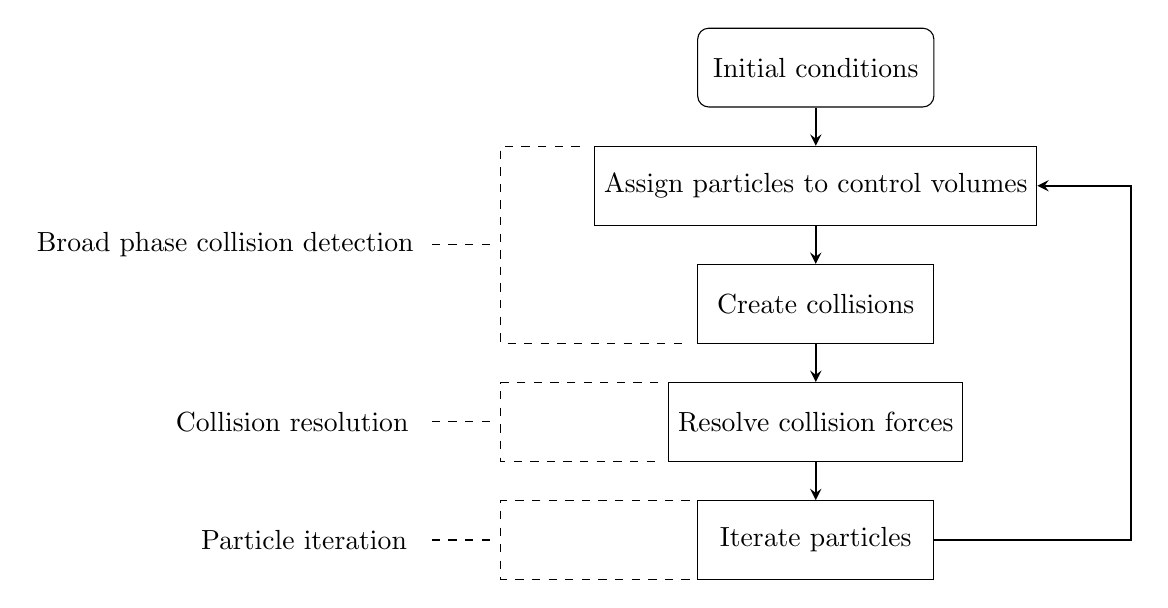
\begin{tikzpicture}
\tikzstyle{startstop} = [rectangle, rounded corners, minimum width=3cm, minimum height=1cm,text centered, draw=black]
\tikzstyle{io} = [trapezium, trapezium left angle=70, trapezium right angle=110, minimum width=3cm, minimum height=1cm, text centered, draw=black]
\tikzstyle{process} = [rectangle, minimum width=3cm, minimum height=1cm, text centered, draw=black]
\tikzstyle{decision} = [diamond, minimum width=3cm, minimum height=1cm, text centered, draw=black]
\tikzstyle{arrow} = [thick,->,>=stealth]

\node [startstop] (v5) at (0,0) {Initial conditions};

\node [process] (v1) at (0,-1.5) {Assign particles to control volumes};
\node [process] (v2) at (0,-3) {Create collisions};
\node [process] (v3) at (0,-4.5) {Resolve collision forces};
\node [process] (v4) at (0,-6) {Iterate particles};
\draw [arrow] (v1) edge (v2);
\draw [arrow] (v2) edge (v3);
\draw [arrow] (v3) edge (v4);
\draw [arrow](v4) -- (4,-6) node [arrow] {} -- (4,-1.5) node [arrow] {} -- (v1);
\draw [arrow] (v5) edge (v1);
\draw [dashed] (-3,-1) -- (-4,-1) -- (-4,-3.5) -- (-1.6,-3.5);
\node (v7) at (-4,-2.25) {};
\node (v6) at (-5,-2.25) {};
\draw [dashed] (v6) edge (v7);
\node at (-7.5,-2.25) {Broad phase collision detection};
\draw [dashed] (-2,-4) -- (-4,-4) -- (-4,-5) -- (-2,-5);
\node (v9) at (-4,-4.5) {};
\node (v8) at (-5,-4.5) {};
\draw [dashed] (v8) edge (v9);
\draw [dashed](-1.6,-5.5) -- (-4,-5.5) -- (-4,-6.5) -- (-1.6,-6.5);
\node (v11) at (-4.,-6) {};
\node (v10) at (-5,-6) {};
\draw [dashed] (v10) edge (v11);
\node at (-6.65,-4.5) {Collision resolution};
\node at (-6.5,-6) {Particle iteration};
\end{tikzpicture}